\let\nofiles\relax
\documentclass[journal]{IEEEtran}
\usepackage[UTF8]{ctex}
\usepackage{bookmark}
\usepackage{hyperref}
\usepackage{graphicx}
\usepackage{xcolor}
\usepackage[thicklines]{cancel}
\usepackage{amsfonts}
\usepackage[justification=centering]{caption}
\graphicspath{ {./images/} }

\begin{document}
\title{Transformer及其在多模态学习方向的扩展}

\author{马筱雅 PB22111639}

\maketitle

\begin{abstract}
Transformer是一种很有前景的神经网络,在很多任务上表现出了优异性能,尤其是在自然语言处理领域。Transformer目前也被用来研究多模态学习。本文调研了Transformer及其在多模态学习方向的扩展,详细介绍了Transformer结构、Transformer和多模态学习结合的模型结构以及模型示例,最后提出了多模态Tranformer面临的挑战并在结论处总结了此次调研的学习心得,。
\end{abstract}

\begin{IEEEkeywords}
Transformer,多模态,注意力机制,模态对齐,模态融合
\end{IEEEkeywords}

\section{Introduction}
多模态数据包含文本、图像、音频等不同类型的数据,是人类社会的重要组成部分。因此,人工智能(AI)作为一种感知与模仿人类的工具,也需要拥有学习和理解多模态数据的能力。近年来,多模态学习(MML)已经成为一个重要的研究领域,也产生了许多相关应用,比如人脸识别等。然而,多模态数据的表现形式多样,相对文本本身更难被计算机理解,也带来了更大的挑战。随着深度学习和神经网络等的发展,AI理解人类语言等的能力显著提高,也为多模态学习带来了新的思路。例如卷积神经网络(CNN)利用卷积核提取图像特征,在许多图像处理任务中表现出色。

Transformer\cite{vaswani2017attention}作为一种深度学习模型,提出了一种新的注意力机制,在自然语言处理(NLP)领域表现出了很优异的性能。鉴于Transformer的优势,Transformer也被扩展应用到多模态学习领域,一系列基于Transformer的多模态模型,例如(ViLBERT\cite{lu2019vilbert},CLIP\cite{radford2021learning})应运而生。本文将调研Transformer及其在多模态学习方向的延伸与应用。

受到\cite{10123038}和ChatGPT的启发,本文从多模态Transformer结构的角度出发,分别从模态对齐和模态融合两方面阐述Transformer和多模态的结合。与\cite{10123038}不同,本文主要从模态交互的角度出发,而\cite{10123038}主要从自注意力机制变体和应用的角度出发调研了多模态Transformer。

综上所述,本文的主要内容包含以下部分:
\begin{enumerate}
\item 在第\ref{Transformer}部分,本文介绍了原始Transformer的结构,并详细解释了其核心组件。
\item 在第\ref{fusion}部分,本文从对比学习、单流结构、多流结构和混合流结构介绍了Transformer在多模态方向的扩展及其实例。
\item 在第\ref{challenge}部分,本文调研了多模态Transformer发展的挑战。
\end{enumerate}

\section{Transformer}\label{Transformer}
Transformer\cite{vaswani2017attention}最初被用来处理序列到序列的任务,它通过注意力机制来构建输入与输出的全局依赖关系。Transformer主要包括编码器和解码器模块,每个模块均有多个层堆叠而成。对于编码器,每个层包含两个子层,第一个子层为多头自注意力层,第二个子层为前馈神经网络层,每一子层中采用残差连接并进行归一化。解码器的每一层多了一个多头自注意力子层,用于处理编码器的输出。图一\ref{figure1}展示了Transformer的基本架构。下面通过几个方面具体介绍Transformer。

\begin{figure}[h]
    \centering
    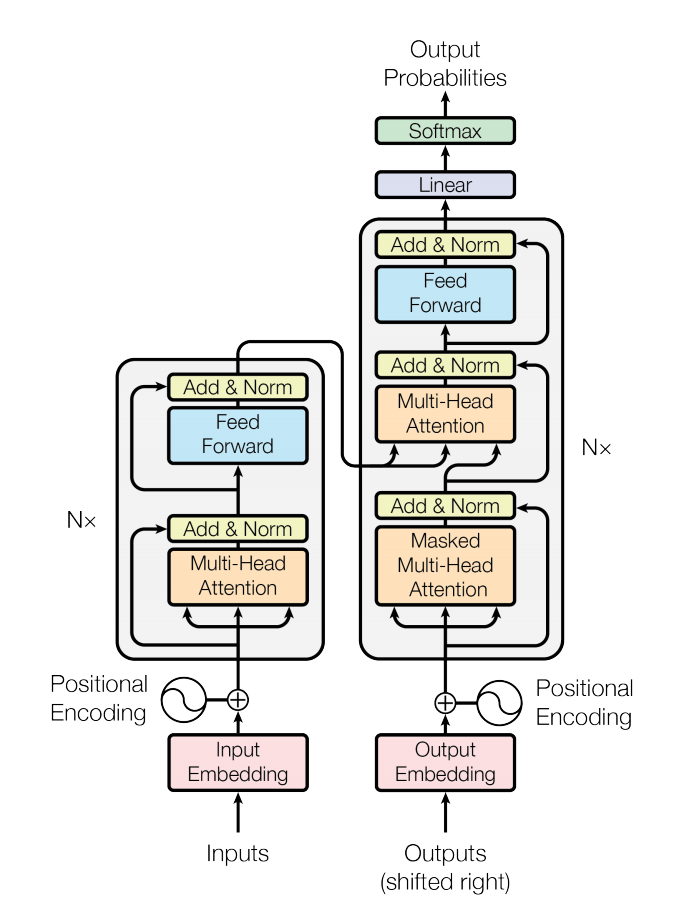
\includegraphics[width=\columnwidth]{image-1.png}
    \caption{Transformer架构}
    \label{figure1}
    \end{figure}

\subsection{注意力机制}
注意力机制中包含三个组件,分别为查询$Q$、键$K$和值$V$。注意力机制中键$K$和值$V$对应,该机制通过某种方式匹配查询$Q$和键$K$,从而对值$V$进行选择。注意力机制是Transformer的核心,主要包括自注意力和多头注意力两个部分。

\subsubsection{自注意力机制}
在卷积神经网络中,由于卷积核大小等的限制,模型很难关注到全局特征,对于循环神经网络由于序列长度等问题同样难以关注全局信息,Transformer通过自注意力机制打破了这一限制。

Transformer首先将输入进行嵌入并结合位置编码得到输入矩阵。假设$Z = [z_1,z_2,...] \in \mathbb R^{N \times d}$作为输入。
在自注意力机制中,$Q$,$K$,$V$来自同一组输入,即此三个矩阵均通过$Z$投射得到($W^Q \in R^{d \times d_q}$,$W^K \in R^{d \times d_k}$, $W^V \in R^{d \times d_v}$,$d_q = d_k$),计算方式为
$Q = ZW^Q$,$K = ZW^K$,$V = ZW^V$ \cite{10123038}。

得到$Q$,$K$,$V$后,通过以下公式计算自注意力
$$Attention(Q,K,V) = \textit{Softmax}(\frac{QK^T}{\sqrt{d_q}}V)$$
直观上看,通过映射得到的$Q$,$K$,$V$,每一行都代表一个输入分词的向量,通过矩阵相乘,使得两个矩阵中每个向量都能和所有向量进行点乘,从而实现了对全局信息的关注。在向量空间中,如果两个向量点乘结果较大,则说明两者距离较近,关联度较高,从而可以计算出$Q$的每个数据与$K$的数据的关联度,关联度高的比重较大。根据计算得到的比重可以对对应$V$中的数据进行加权选择。

在解码器中,Transformer还采用掩码自注意力的形式,这种方式能够帮助Transformer学习上下文依赖,具体方式为
$$Mask-Attention(Q,K,V)=\textit{Softmax}(\frac{QK^T}{\sqrt{d_q}}\bigodot M)V$$
其中$M$是掩码矩阵。

\subsubsection{多头注意力机制}
Transformer通过利用不同的投射机制,把输入$Z$映射到多个$Q$,$K$,$V$中,每一组$Q$,$K$,$V$的注意力输出作为一个注意力头。对得到的多个注意力头进行拼接,再次进行映射得到最终的$Q$,$K$,$V$矩阵,进而计算注意力。如图二\ref*{figure2}所示。直观上看,每个输入可能包含多个信息,单注意力将输入投射到一个特征空间,从而导致对信息的提取不充分。多头注意力将输入投射到多个特征空间,每个特征空间对输入信息侧重点不同,从而提取出更多的信息,表意更充分,带来更好的性能。
\begin{figure}[h]
    \centering
    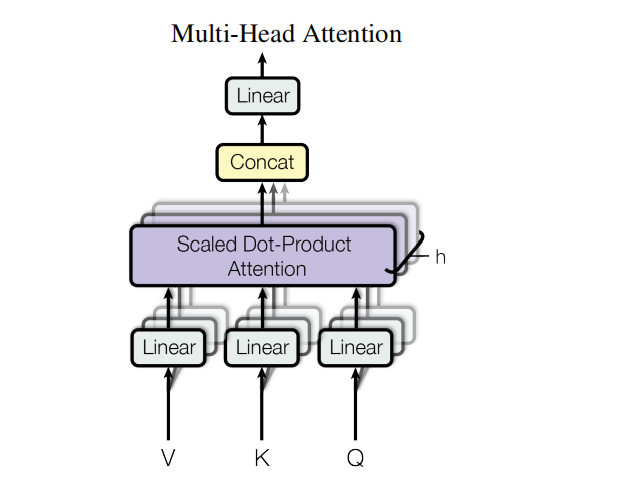
\includegraphics[width=\columnwidth]{image.png}
    \caption{多头注意力机制}
    \label{figure2}
    \end{figure}

\subsection{位置编码}
对于输入序列,Transformer会对输入进行嵌入后整合位置信息,从而能够考虑到不同位置带来的信息差异。Transformer采用类似于傅里叶变换的形式,采用$sin$和$cos$函数进行位置编码。
$$PE_{(pos,2i)} = sin(pos/10000^{2i/d_{model}})$$ 
$$PE_{(pos,2i+1)} = cos(pos/10000^{2i/d_{model}})$$ 
其中$d_{model}$是指输入数据进行嵌入后的维度。直观上看,如果没有位置编码,对于一个输入序列,比如说“牛奶”和“奶牛”就会被编码为相同的向量。对位置信息的编码使得Transformer能更好地捕捉语义的上下文关联。

\subsection{前馈神经网络(FNN)}
前馈神经网络由线性变换函数和非线性激活函数构成。例如,该层可以用数学公式表示为
$$FFN(Z) = \sigma (ZW_1 + b_1)W_2 + b_2$$
其中$W_1$, $W_2$是权重,$b_1$,$b_2$是偏差,$\sigma$ 是激活函数。该层可以进行特征变化,通过非线性变换映射到不同的特征空间,捕获更复杂的特征和形式。


\section{多模态Transformer}\label{fusion}
与单模态数据不同,多模态数据的表现形式复杂且不统一,不同模态数据有不同的特点,所以对于不同模态数据的处理方式不同。不同的处理方式可能导致不同的处理结果,比如,表示同种含义的文本和图片可能具有不同的向量表示,进而带来了模态对齐与模态融合的主要问题。模态对齐,是指不同模态中表达相同或相似信息的数据在特征空间中具有一致的表示;模态融合是指将来自不同模态的特征整合在一起,为信息构建统一表示。下文从对比学习的角度调研了结合Transformer进行模态对齐的方式,从单流、多流和混合流的角度调研了结合Transformer进行模态融合的方式。

\subsection{对比学习}
对比学习通过最大化相关样本的相似度和最小化无关样本的相似度来提取有意义的特征,在此过程中,规定了正负样本,相关的样本为正样本,不相关的是负样本。在多模态对齐中,要使表示相同含义的多模态数据有相同的数据表示,可以通过对比学习的方式,比如最大化相关的图片和文本之间的向量相似度,最小化无关的图片和文本之间的向量相似度,从而使得表示相同含义的不同模态的数据具有相同的表示。将对比学习与Transformer结合,一方面利用了对比学习进行模态对齐的思想,另一方面利用了Transformer的编码能力等,为多模态学习提供了新的思路。

CLIP\cite{radford2021learning}是一个典型的基于对比学习进行模态对齐的多模态Transformer架构。CLIP通过文本编码器编码文本数据,通过图像编码器编码图像数据。CLIP对于Transformer的应用体现在其编码器上。CLIP的图像编码器架构使用了Vison Transformer(ViT)\cite{dosovitskiy2020image},这是Transformer的一种处理图像任务的模型变体。ViT首先把图像划分为固定大小的块,由于图像不是二维数据,则通过一个嵌入层将其转换为二维数据并附加上不同图像块的位置编码信息,最后调用一个标准的Transformer编码器进行编码。CLIP的文本编码器同样基于Transformer架构。CLIP基于一组关联相关图像和文本的数据集训练模型。通过利用Transformer对图像和文本同时编码并进行相关性计算,对比学习增强相关文本与图像之间的关联度,促进了多模态的模态对齐,是一个Transformer用于多模态的重要实例。

\subsection{单流结构Transformer}
单流结构是指不同模态的数据经表征后被映射到相同的特征空间,之后作为Transformer的输入,利用单一Transformer对多模态数据进行训练。在训练过程中,每一层的注意力交互都可以关注到模态内和模态间的完整上下文,从而进行模态融合。鉴于不同模态数据结合的时间较早,这种方式也被称为早期融合。\cite{10123038}对于不同模态数据的组合,有多种方式,常见的有将图像向量和文本向量进行简单相加或者拼接。

UNITER模型是该结构的典型代表,下面以该模型为例具体调研单流结构Transformer。UNITER\cite{2020UNITER}主要对图像和文本数据进行处理。对于图像数据,UNITER使用图像嵌入器进行图像向量化,对于文本数据,UNITER采用文本嵌入器进行进行文本向量化,通过两种嵌入器将多模态数据映射到相同维度的向量空间,得到的向量直接作为Transformer编码器的输入。在训练过程中,利用Transformer的自注意力机制和前馈神经网络层结构等学习跨模态上下文。此模型通过多层Transformer对多种跨模态任务进行预训练,在图像+文本任务上表现出了优异的性能。

单流结构Transformer中不同模态数据共享权重,统一进行训练,可以进行跨模态或者模态间的交互,是一种常见的使用Transformer处理多模态数据的方式。

\subsection{多流结构Transformer}
对于单流结构Transformer,不同模态信息的早期融合可能导致单一模态内部学习不充分,也有可能在训练过程中过分关注单一模态,导致模态间学习不充分。于是存在多流结构Transformer,既进行模态内特征提取,又进行跨模态交互。多流结构Transformer是指不同模态的数据流通过各自的Transformer编码器捕获特征,之后通过一定的跨模态交互机制来融合不同模态的信息。对于不同模态数据的跨模态交互,多流结构Transformer引入了一种交叉注意力机制。

交叉注意力机制在\cite{lu2019vilbert}中提出。标准的Transformer层采用自注意力机制,$Q$,$K$,$V$来自同一组输入,而在交叉注意力机制中,来自不同模态的$Q$,$K$,$V$彼此互相交换,作为Transformer层的输入。假设$Q_v$,$K_v$,$V_v$来自图像,$Q_w$,$K_w$,$V_w$来自文本,则有
$$Attention_{(V)} = MHSA(Q_w,K_v,V_v)$$
$$Attention_{(W)} = MHSA(Q_v,K_w,V_w)$$
其中$MHSA$指代多头自注意力(Multi Head Self-Attention)。通过交叉注意力机制,Transformer能够基于其他模态来关注当前模态,从而促进了跨模态的交互和融合。

ViLBERT和LXMERT是典型的基于多流架构的多模态Transformer架构,以该两种模型为例,具体调研多流Transformer。

\subsubsection{ViLBERT}
ViLBER\cite{lu2019vilbert}包含两个并行的数据流,一个用于处理图像数据,一个用于处理文本数据。首先分别用图像和文本嵌入器对图像和文本进行嵌入得到向量表示。每一个流结构包含k个Transformer层和交叉注意力Transformer层组成的块,进行跨模态交互。在此之前,对于文本流数据,首先对文本向量采用独立的Transformer模块对单模态数据进行训练,从而进行模态内部特征的提取。ViLBERT有效结合了模态内和跨模态的信息提取,有助于处理多模态数据。但是没有实现对图像流数据进行单模态训练,LXMERT改善了这一问题。

\subsubsection{LXMERT}
LXMERT\cite{tan2019lxmert}构建了三个编码器,包含一个语言编码器,对象关系编码器和一个跨模态编码器。语言编码器和对象关系编码器均是单模态编码器,分别用来处理文本和图像数据,且均由一个自注意力子层和前馈网络子层构成,类似于Transformer编码器结构。通过多个连续的单模态编码器提取模态内信息。与ViLBERT不同,ViLBERT只对文本进行单模态编码,而LXMERT对图像和文本均进行单模态特征提取。数据流经过单模态编码器后通过跨模态编码器训练。跨模态编码器由一个交叉注意力子层,一个自注意力子层和一个前馈层构成,类似于交叉注意力层和Transformer编码器层结合。通过跨模态编码器可以用来交换不同模态的信息并且可以学习联合跨模态表征,从而促进数据的跨模态学习和融合。

多流结构既关注了模态内信息,也关注了模态间信息。通过运用不同深度的跨模态编码器进行训练,也可以灵活地对每个模态特征进行不同深度的提取。由于堆叠的注意力层较多,多流结构Transformer的参数量较大,计算成本较高,由于跨模态Transformer层数有限,不同模态交互也有限。

\subsection{混合流结构Transformer}
单流结构Transformer和多流结构Transformer各有优缺点,因此混合流结构将两种方式结合,主要通过多流到单流的方式。多流到单流的Transformer结构前半部分通过对不同模态的数据进行单一模态编码并利用交叉注意力进行跨模态编码,后半部分将不同模态的数据通过相加或拼接等方式结合在一起,再次进行训练。这种方式即关注了单模态表征学习,也关注了深层的模态融合,模态交互的深度增加,但模型结构更为复杂。

综上,多模态Transformer主要利用了Transformer的编码器等结构,通过Transformer的注意力机制及其变体(如交叉注意力)来对多模态数据进行训练,从而对多模态数据进行深层次的特征提取。通过单流、多流和混合流的Transformer结构和对比学习等方式,Transformer有效助力了多模态学习。

\section{多模态Transformer的挑战}\label{challenge}

如上文所述,模态对齐和融合是多模态Transformer的重要研究问题,也是多模态Transformer的重大挑战。除此之外,本文还调研了其他多模态Transformer面临的挑战,包含包括通用性问题和模型开销问题。
\subsection{通用性} 多模态场景下具有许多不同类型的任务,比如说图像生成,图像识别、视频理解分析、音频理解等,所以构建一个通用Transformer的挑战很大。理想情况下,统一的多模态Transformer可以兼容各种数据(如对齐和非对齐、单模态和多模态)和任务(如监督和无监督、单模态和多模态、鉴别和生成),同时具有少量甚至零样本的泛化能力。\cite{10123038}。目前,由于训练所用的数据集不同和模型构造不同,不同的多模态Transformer的适用的场景不同。比如,CLIP适用于图像分类、图像检索等问题,VideoBERT适用于视频描述等任务。因此,构建通用能力强的多模态Transformer模型还具有很大的发展空间。
\subsection{模型开销} 根据\cite{vaswani2017attention},对于单层自注意力结构,层复杂度就达到了$O(n^2d)$,其中$n$是输入序列的长度,$d$是表征向量的维度。通过单流,双流和混合流的多模态Transformer结构可以看出,多模态Transformer对Transformer等结构的堆叠层数层数较多,模型参数量巨大,因而带来了较大的计算和存储开销。此外,由于多模态数据的特殊性,在模型训练阶段需要大量的数据,也带来了较大的资源开销和效率问题。\cite{10123038}详细列举了提高模型效率的方案。


\section{Conclusions}
本文调研了Transformer及其在多模态方向的扩展及挑战。首先调研了Transformer的结构及其主要思想,接着从模态对齐和模态融合两个方面调研了Transformer在多模态学习方面的扩展方式,并调研了每一种设计结构的代表模型。最终从模型通用性和开销两个方面讨论了多模态Transformer面临的发展挑战。

\subsection{学习心得}
在本次调研任务中,我首先确定了调研主体是Transformer模型,先细致看了"All Attention is All You Need"这篇文章,接着看了一篇关于Transformer的综述。由于我对多模态任务比较感兴趣,就联想到了Transformer在多模态方面的扩展。于是我首先查找了关于多模态Transformer的论文,发现有一篇关于多模态Transformer的综述,通过这篇综述,我对多模态Transformer有了一个大致的了解。为了防止和该综述重合,我通过ChatGPT和各种博客,调研了关于多模态Transformer的结构和值得研究的方向,最终决定主要从模态融合与对齐的角度出发。
在调研过程中,我通过检索论文和阅读论文博客等大致了解了模态融合和对齐及多模态Transformer模型的典型代表。在写报告过程中,我不断思考模态对齐融合和多模态Transformer这个主题的关联,感觉调研的内容有些局限,但又由于已经有综述存在,又不想和已有的综述角度重合,一度陷入了混乱。最终不断调整思路,把内容和多模态Transformer靠拢。

通过本次调研,我详细学习了Transformer的结构及其设计的原理,对其设计原因进行了思考,并对Transformer在多模态任务上的利用有了一个宏观的了解,但对微观上的细节问题还是了解不够深入,需要更深刻的体会。同时,我也通过实际操作学到了阅读论文,总结论文,调研论文的方式,以及使用latex编写论文的方法。除此之外,我也丰富了在调研过程中一步步明确自己的目的,细化自己的需求,并和已有文章进行横向比较的经验。

\appendices

\bibliographystyle{plain} % We choose the "plain" reference style
\bibliography{refs}


\end{document}


